\chapter{Testování}

% \begin{itemize}
%  \item Způsob, průběh a~výsledky testování.
%  \item Srovnání s~existujícími řešeními, pokud jsou známy.
% \end{itemize} 

\section{Uživatelské testování}
Uživatelské testování bylo prováděno za přítomnosti kolegy z~projektového týmu a uživatele - testera, který byl ochoten věnovat dvě hodiny svého času testování. Popis testování linuxové části byl zde vypuštěn.

\subsection{Zadání}
Uživatel měl za úkol otestovat aplikaci v~několika krocích:
\begin{enumerate}
 \item spuštění serveru a připojení klientů pomocí skriptů, uživatel měl k~dispozici textový soubor \verb|readme.txt| s~informacemi o~spuštění
 \item kontrola průchodů všech módů Cisco IOS + testování nestandartních vstupů
 \item konfigurace rozhraní
 \item konfigurace statického překladu adres na počítači \verb|cisco1| pro \verb|linux1|
 \item konfigurace dynamického překladu adres na počítači \verb|cisco1| pro \verb|linux2|
\end{enumerate}

Na obrázku \ref{fig:testovani} je znázorněno zadání, které dostal uživatel. Uživatel postupoval dle zadání a pomocí tohoto obrázku konfiguroval síť.

\begin{figure}[h]
\begin{center}
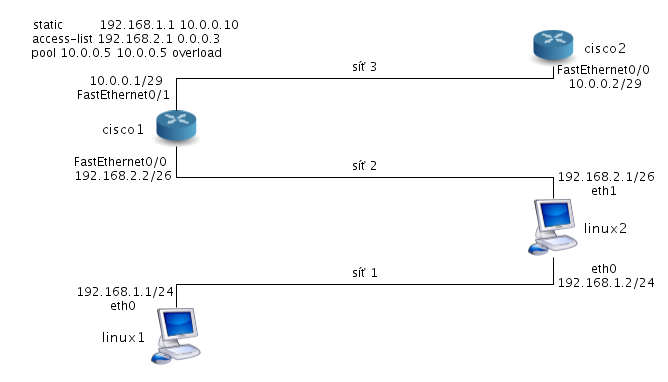
\includegraphics[width=15cm]{figures/testovani}
\caption{Zadání sítě pro uživatelské testování}
\label{fig:testovani}
\end{center}
\end{figure}


\subsection{Průběh testování}
U~každé objevené chyby bude vyznačeno tučným písmem implementované řešení problému či alespoň komentář s~vysvětlením. 

\subsubsection{Úkol č.1 spuštění serveru}
Uživatel byl znalý linuxu, a tak pro spuštění serveru zkusil příkaz:
\begin{verbatim}
./start_server.sh --help
\end{verbatim}
Skript však reaguje pouze na spuštění bez parametru a na parametr \verb|-h|. Tudíž se spustil server s~konfiguračním souborem \verb|--help| a vypsal chybu, že nelze nic načíst z~takového souboru.
\\\textbf{(volba --help přidána)}

Uživatel zkusil spustit server na obsazeném portu. Aplikace vypsala chybovou nepříliš jasnou hlášku.
\\\textbf{(chybová hláška přidána)}

Klientský skript pro připojení k~serveru nevypsal chybovou hlášku, když nebyl specifikován port (= virtuální počítač).
\\\textbf{(chybová hláška přidána)}

\subsubsection{Úkol č.2 průchod stavy IOS}
Server vypisuje různé důležité (průchod paketu - směrování, překlad adres) informace. Server ale také vypisuje všechny přijaté a odeslané příkazy, které činí výpis velmi nepřehledným.
\\\textbf{(nedůležité výpisy odstraněny)}

Uživatel zaznamenal, že při procházení historií příkazů (pomocí šipek nahoru a dolu) se nabízejí příkazy i z~jiných terminálů - linux i cisco najednou. Navíc si pamatuje příkazy i po znovu spuštění klienta.
\\\textbf{(daň za použití programu třetí strany)}

Pomocný příkaz \verb|help| reps. \verb|help_en| není nikde v~\verb|readme.txt| zveřejněn, takže uživatel neznal podporované příkazy.
\\\textbf{(informace o~příkazu help přidána do readme.txt)}

Uživatel našel bug\footnote{chyba v~programu} při přechodu z~privilegovaného do konfiguračního stavu. Při \verb|configure memory| se přeplo cisco do \verb|configure terminal|.
\\\textbf{(chyba opravena)}

\subsubsection{Úkol č.3 nastavení rozhraní}
Při konfiguraci síťových rozhraních se přišlo na jednu závažnou chybu. Při nastavování IP adresy zadal uživatel neplatnou masku a program vyhodil výjimku.
\\\textbf{(zpracování chybných adres bylo při testování hotové, ale v~implementaci chyběl příkaz return pro vyskočení z~metody při odchycení výjimky)}

\subsubsection{Úkol č.4 směrování}
Konfigurace smětovacích záznamů odhalila jednu chybu či spíše \uv{nedodělek}. Spuštěný příkaz \verb|ping| bez parametrů nedělá vůbec nic (žádná chybová hláška ani správna funkcionalita).
\\\textbf{(ping bez parametrů vypíše vysvětlující informaci)}

\subsubsection{Úkol č.5 statický NAT}
Do zadání statického NATu byla předem vložena chyba, aby se oveřilo, zda se aplikace bude správně chovat. Adresa \verb|192.168.1.1| se měla přeložit na \verb|10.0.0.10|, ta ale nespadá do sítě č.3, a tak \verb|cisco2| nevědělo, kam má paket s~odpovědí poslat.

Po změně překladu \verb|192.168.1.1| na \verb|10.0.0.6| (poslední volná IP adresa sítě č.3) už pakety bez problému došly.

\subsubsection{Úkol č.6 dynamický NAT}
Uživatel zkoušel postupně přidávat pravidla pro access-list a pool. Příkaz \verb|access-list| bez parametru měl vypsat hlášku \verb|Incomplete Command.|, ale nic nevypsal.
\\\textbf{(přidán výpis do parseru příkazu)}

Po nakonfigurování dynamického NAT zkoušel uživatel dostupnost jednotlivých počítačů přes příkaz \verb|ping|. Uživatel přidal do linuxových počítačů defaultní směrovací záznamy na \verb|cisco2|. Do routovací tabulky na \verb|cisco2| se vůbec nezasahovalo (vyjma automaticky nastaveného záznamu na rozhraní). Příkazem ping byla ověřena dostupnost \verb|cisco2| z~obou linuxových počítačů. Naopak \verb|ping 10.0.0.5| z~\verb|cisco2| nezafungoval, protože \verb|linux1| je skryt za NATem a paket by musel být odeslán se správným portem z~NAT tabulky. Cisco IOS u~příkazu \verb|ping| neumožňuje měnit číslo portu u~odesílaného paketu.


%\\\textbf{()}

\subsection{Shrnutí}
Z~počtu chyb lze jasně vyvodit, že uživatelské testování určitě smysl má. Většinu objevených chyb tvoří různé chyby či odchylky v~parserech.





\section{Zátěžové testy}\label{zatezove_testy}

\subsection{Návrh}

\subsection{Výsledky}

